\section{Geometric Analyses} \label{sec:geometric}

In this section, we consider the geometry that tag matching metrics impose over bitstring tag space.
Geometric constraints of tag matching metrics may affect the patterns of tag connectivity that tend to (or even are possible to) arise under a tag-matching metric. %TODO
For example, in metrics with strong geometric constraints, sets of tags may exist such that no single tag can simultaneously exhibit a close affinity to more than one tag in the set.
Likewise, under metrics with strong geometric constraints, a set of tags may exist such that any tag must ither match all tags in the set well or match all tags in the set poorly.
Geometric constraint might prove useful to facilitate modularity, where subsets of tag space tend to have associated functionality.
However, it may also restrict the generation of adaptive variation.

We compare distributions of two statistics measuring constraint across our five tag-matching metrics: similarity constraint and dissimilarity constraint.
% \begin{figure}
\begin{center}

\begin{subfigure}[b]{0.5\linewidth}
\centering
\includegraphics[width=\linewidth]{dimensionality-statistic}
\caption{
Dimensionality statistic
}
\label{fig:dimensionality_statistic}
\end{subfigure}%
\begin{subfigure}[b]{0.5\linewidth}
\centering
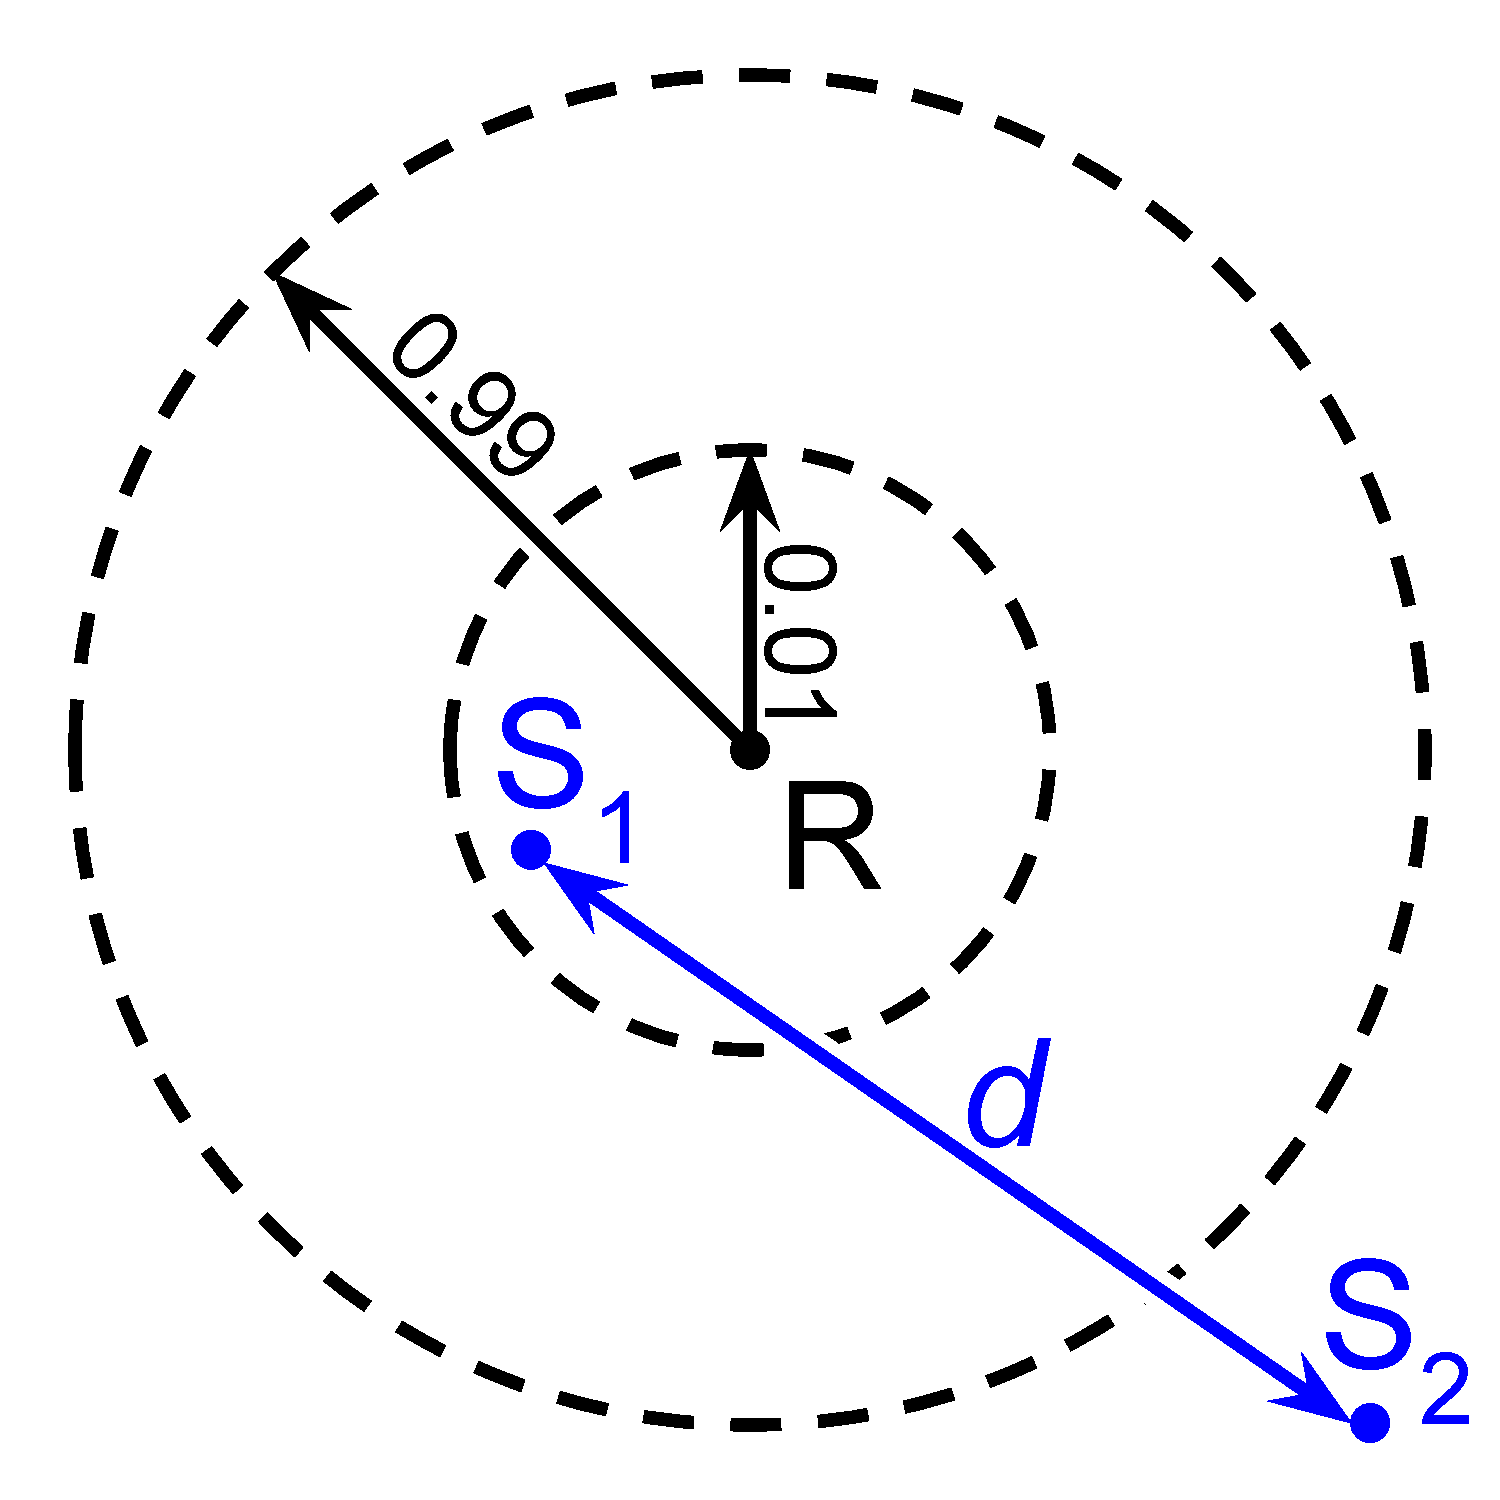
\includegraphics[width=\linewidth]{elasticity-statistic}
\caption{
Elsaticity statistic
}
\label{fig:elasticity_statistic}
\end{subfigure}

\caption{
A schematic depicting (A) the process used to generate the dimensionality statistic for each metric and (B) the process used to generate the elasticity statistic for each metric.
}
\label{fig:dimensionality_measure}

\end{center}
\end{figure}

Similarity constraint quantifies the question, "If two tags both match closely to a third tag, will they necessarily match closely with each other?"
To compute this statistic, we randomly sampled 5000 target tags.
Then, for each target tag we randomly sampled tags until we found two secondarily-sampled tags that were within a 0.01 match distance radius to the target.
Finally, we computed the match distance between the pair of secondarily-sampled tags.
Figure \ref{fig:dimensionality_measure} summarizes this process.

Dissimilarity constraint quantifies the question, ``If a tag matches a second tag closely and a third tag poorly, will the second and third tag tend to match poorly?"
Analysis of this statistic, which yielded results closely mirroring the similarity constraint statistic, is provided in \href{doi.org/10.17605/OSF.IO/GW5MC}{Supplementary Section \ref{sec:dissimilarityconstraint}} \cite{Moreno_Ofria_2020}.

\subsection{Similarity Constraint}

\begin{figure*}
\begin{center}

\begin{minipage}{\linewidth}
\begin{subfigure}[b]{\linewidth}
\begin{minipage}{0.5\textwidth}
\begin{center}
\includegraphics[width=0.5\linewidth,trim=5cm 5cm 5cm 5cm, clip]{img/dimensionality-statistic}
\end{center}
\end{minipage}%
\begin{minipage}{0.5\textwidth}
\caption{
Sampling process used to measure similarity constraint.
First, a constraining tag $R$ was randomly sampled.
Then, tags were randomly drawn until two tags $S_1$ and $S_2$ with distance to $R$ less than 0.01 were obtained.
Finally, similarity constraint was measured as the distance $d$ between $S_1$ and $S_2$.
}
\label{fig:dimensionality_measure}
\end{minipage}
\end{subfigure}
\end{minipage}
\begin{subfigure}[b]{\linewidth}
\begin{minipage}{0.6\linewidth}
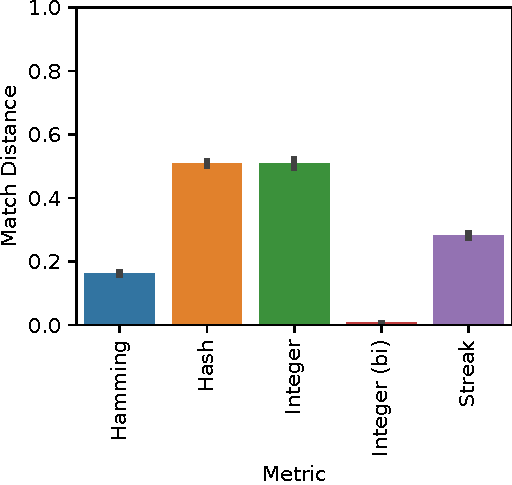
\includegraphics[width=\linewidth]{img/sphere/bitweight=0dot5+seed=1+title=dimensionality_barplot+_data_hathash_hash=c0f6c5cf854ff253+_script_fullcat_hash=03ce1e318a24a109+ext=}
\end{minipage}
\begin{minipage}{0.35\linewidth}
\caption{
Mean similarity constraint.
Error bars represent 95\% confidence intervals.
}
\label{fig:sphere_barplot}
\end{minipage}
\end{subfigure}
\begin{minipage}{\linewidth}
\begin{subfigure}[b]{\linewidth}
\centering
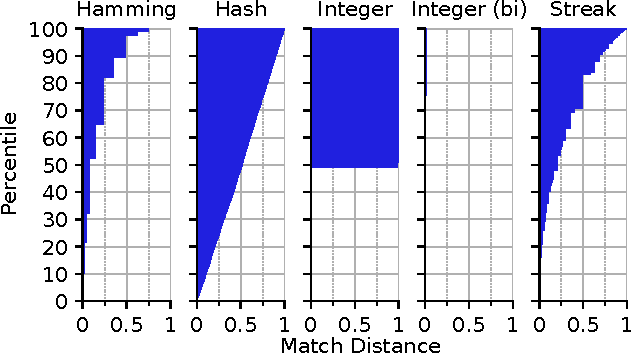
\includegraphics[width=\linewidth]{img/sphere/bitweight=0dot5+seed=1+title=dimensionality_distnplot+_data_hathash_hash=c0f6c5cf854ff253+_script_fullcat_hash=bea2a31376bf6bd0+ext=}
\begin{minipage}{0.8\textwidth}
\caption{
Distributions of sampled similarity constraint values.
Each visualization arranges individually sampled observations (thin horizontal bars) vertically in descending order.
The $y$ axis can be interpreted as ranging form the \nth{0} percentile of outcomes (bottom) to \nth{100} percentile (top) with horizontal bar width showing similarity constraint at a certain percentile.
}
\label{fig:sphere_distnplot}
\end{minipage}
\end{subfigure}
\end{minipage}

\caption{
Similarity constraint of tag-matching metrics.
Figure \ref{fig:dimensionality_measure} summarizes the sampling process used to measure similarity constraint.
Figures \ref{fig:sphere_barplot} and \ref{fig:sphere_distnplot} compare distributions of similarity constraint across metrics.
}
\label{fig:sphere}

\end{center}
\end{figure*}


% In a Euclidean space, similarity constraint corresponds to the average distance between points uniformly sampled from inside a ball (\textit{e.g.}, in two dimensions a circle, in three dimensions a sphere, \textit{etc.}).
% In Euclidean space, this average distance increases with dimensionality.
% For reference, in a one-dimensional Euclidean space similarity constraint would measure approximately 0.0067.
% In a two dimensional Euclidean space, it would measure approximately  0.0091.
% In 32 dimensions, it would measure 0.0137 \citep{dunbar1997average}.

Figure \ref{fig:sphere_barplot} provides our estimate of the similarity constraint statistic for each metric, with error bars representing a 95\% confidence interval.
Figure \ref{fig:sphere_distnplot} shows the distribution of the similarity constraint statistic values among the 5000 replicate samples in greater detail.

For the bidirectional integer metric, we measured the similarity constraint statistic as 0.0068.
This falls in line with expectation: this metric is essentially identical to a one-dimensional Euclidean space.
As shown in Figure \ref{fig:sphere_distnplot}, the secondarily-sampled match distances are all bounded by the diameter of 0.02.
This metric not only exhibits tight similarity constraint in the mean case, but also permits no outliers to the similarity constraint.

The unidirectional integer metric exhibits much looser similarity constraint in the mean case.
We estimated this value as 0.5092.
However, this looser similarity constraint appears to be an artifact of averaging between two very tight constraints: a tight constraint to 0 in one case and a tight constraint to 1 in the other.
Figure \ref{fig:sphere_distnplot} shows that all sampled match distances fall under one of these umbrellas.
Because of the asymmetrical definition of the integer metric, half of pairs of similar scalar values will be in ascending order (resulting in a match distance close to 0) and half will be in descending order, (resulting in a wraparound search and a match distance close to 1).
The integer metric appears to allow for closely related tags to either very strongly match or very weakly match, but permits no intermediate outcomes.

The hamming metric exhibits a broader range of sampled similarity constraint values than the integer metrics.
We estimated mean similarity constraint as 0.1627, looser than the bidirectional integer metric.
As shown in Figure \ref{fig:sphere_distnplot}, many secondarily-sampled tag pairs are biased towards low match distances.
However, secondarily-sampled tag pairs that break this constraint are also not uncommon.
Among our 5000 trials, we observed distances between secondarily-sampled tags as high as 0.7499.

% Why is our estimate of the hamming metric similarity constraint so much higher than the expected value of 0.0137 in a 32-dimensional Euclidean space?
% This phenomenon appears to be due to the normalization process we applied to map raw match distances to a uniform distribution.
% We also calculated this statistic for the raw hamming metric without normalization, increasing the radius of our sampling ball to 0.25.
% (Only an exact target 32-bit tag itself falls within a sampling radius of 0.01.)
% The \textit{a priori} expected distance between sampled points within a 32-dimensional ball with radius 0.25 is 0.3415.
% Our estimate of similarity constraint for the raw hamming metric falls nearly in line with expectation at 0.3312.

The streak metric exhibited the next-loosest similarity constraint statistic with a mean value sampled at 0.2813.
For this metric, we observed distances between secondarily-sampled tags as high as 0.9993.
The streak metric retains some geometric constraint in the mean case, but allows for outliers that strongly break similarity constraint.

Like the unidirectional integer metric, the hash metric also exhibits a very loose similarity constraint of 0.5083 in the mean case.
However, unlike the integer metric, secondarily-sampled match distances are uniformly distributed between 0 and 1.
% This is exactly as we would expect:
% given any particular set of operands, a well-behaved hash function should yield a uniform distribution of hash results.
As expected, the hash metric exhibits no geometric structure.

\subsection{Dissimilarity Constraint} \label{sec:dissimilarityconstraint}

\begin{figure}
\begin{center}

\begin{subfigure}[b]{\columnwidth}
\centering
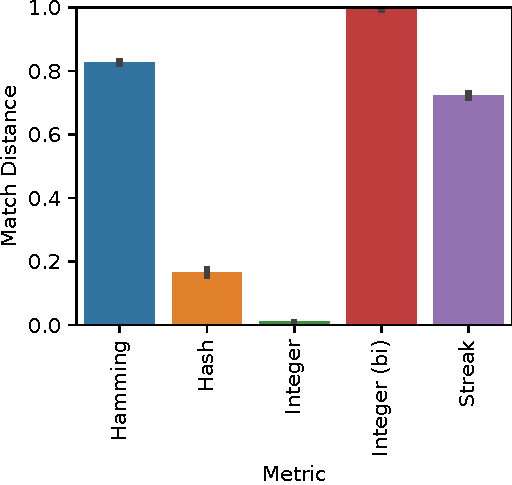
\includegraphics[width=\columnwidth]{{{sphere_reverse/bitweight=0.5+seed=1+title=dimensionality_barplot+_data_hathash_hash=7eaa832497d2f3cb+_script_fullcat_hash=03ce1e318a24a109+ext=}}}
\caption{
TODO
}
\label{fig:sphere_reverse_distnplot}
\end{subfigure}


\begin{subfigure}[b]{\columnwidth}
\centering
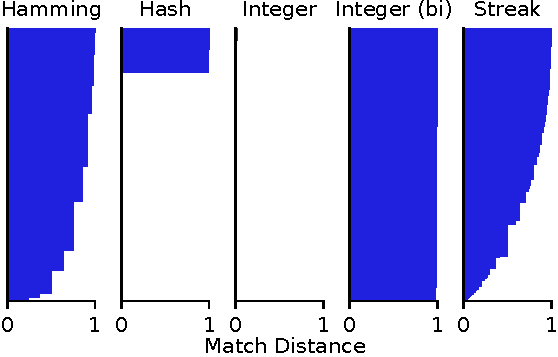
\includegraphics[width=\columnwidth]{{{sphere_reverse/bitweight=0.5+seed=1+title=dimensionality_distnplot+_data_hathash_hash=7eaa832497d2f3cb+_script_fullcat_hash=03ce1e318a24a109+ext=}}}
\caption{
TODO
}
\label{fig:sphere_reverse_barplot}
\end{subfigure}

\caption{
TODO
}
\label{fig:sphere_reverse}

\end{center}
\end{figure}

% \begin{figure}
\begin{center}

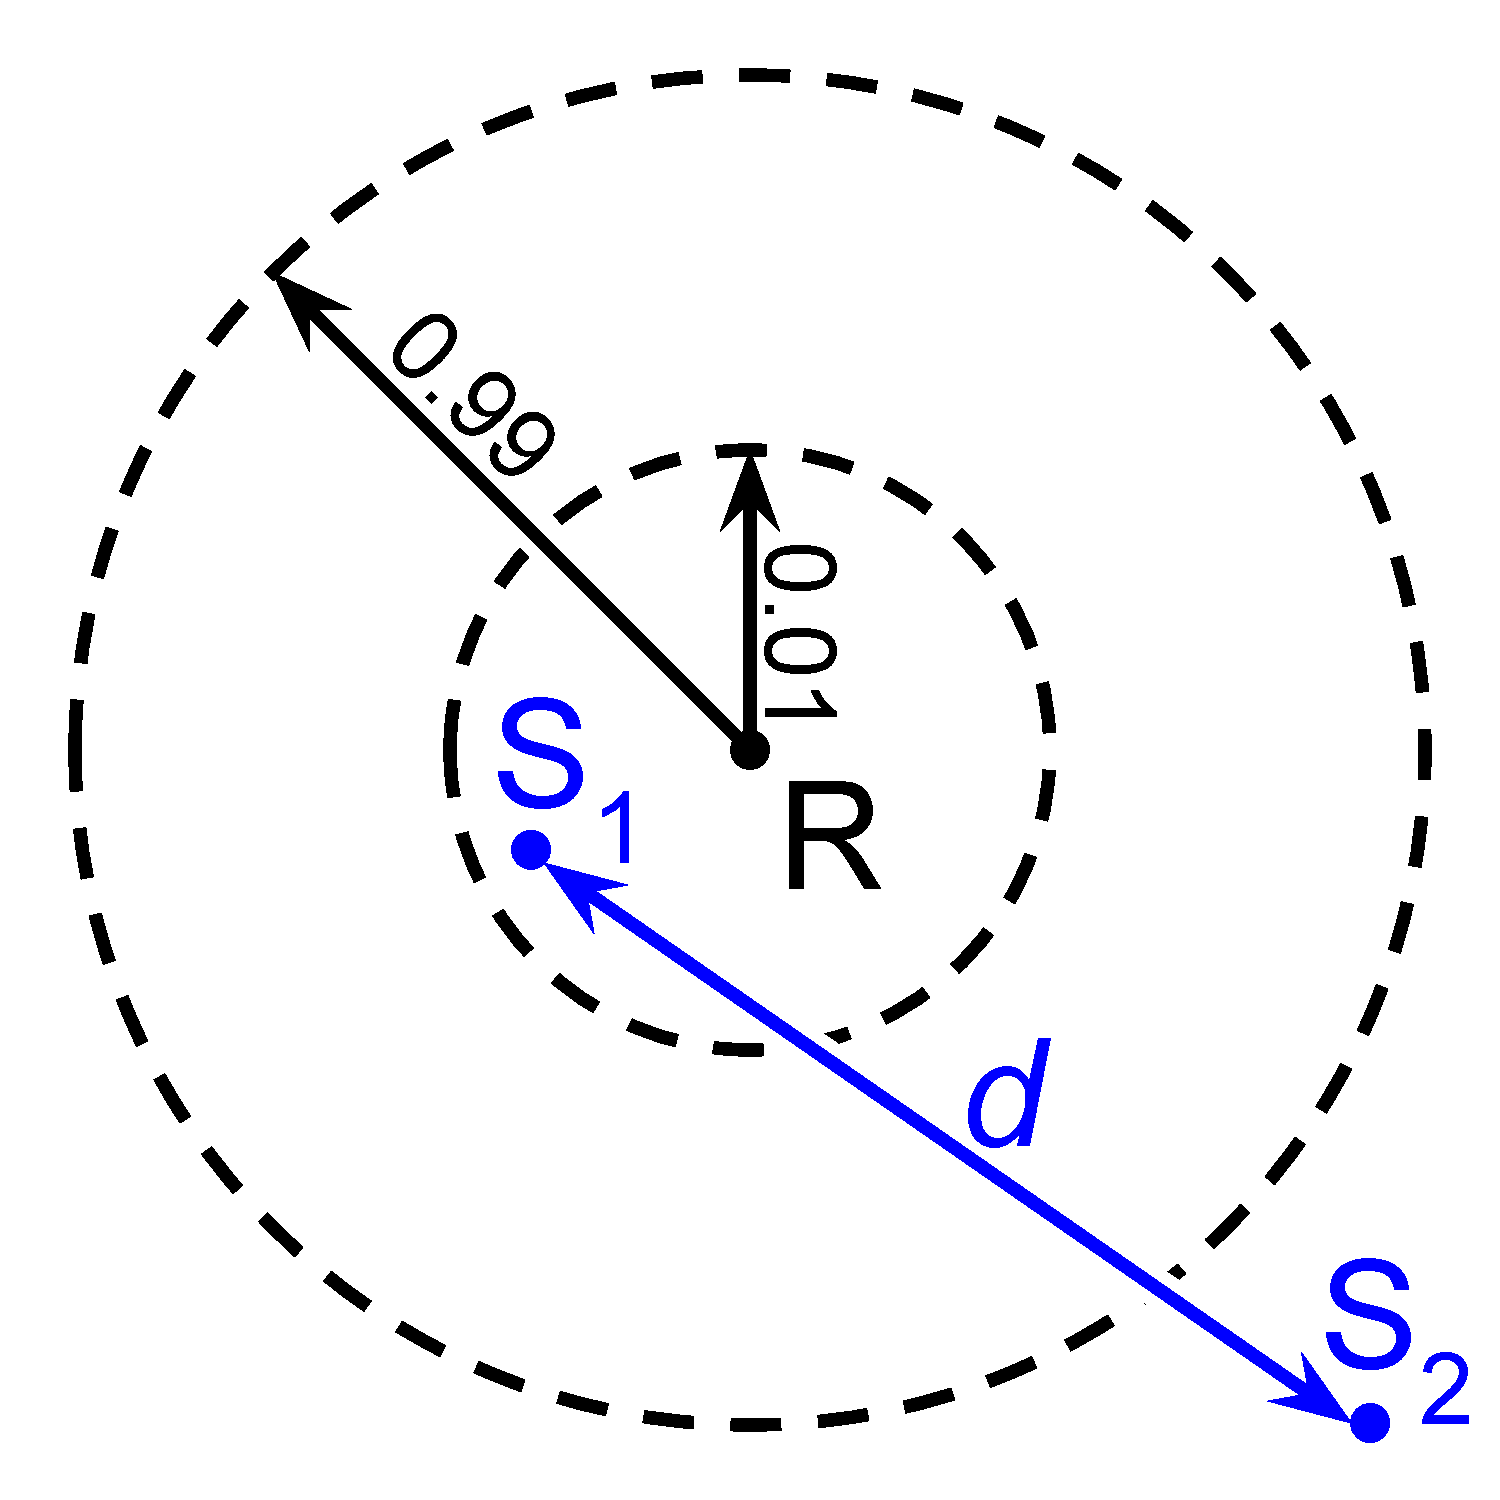
\includegraphics[width=0.5\linewidth]{elasticity-statistic}
\caption{
Dissimilarity statistic
}

\caption{
A schematic depicting the process used to generate the dissimilarity statistic for each metric.
}
\label{fig:dissimilarity_statistic}

\end{center}
\end{figure}


To compute this statistic, we randomly sampled 5000 target tags.
Then, for each target tag we randomly sampled tags until we found a secondarily-sampled tag that was within a 0.01 match distance radius of the target and a secondarily-sampled tag that was outside a 0.99 match distance radius of the target.
Finally, we computed the match distance between the pair of secondarily-sampled tags.
Figure \ref{fig:dissimilarity_statistic} summarizes this process.

Supplementary Figure \ref{fig:sphere_barplot} provides our estimate of the dissimilarity constraint statistic for each metric, with error bars representing a 95\% confidence interval.
Supplementary Figure \ref{fig:sphere_distnplot} shows the distribution of the dissimilarity constraint statistic values among the 5000 replicate samples in greater detail.

These results tell a story across metrics very to the simiarity constraint results.
The hash metric exhibited no geometric structure.
The streak metric exhibited some geometric structure in the mean case (mean secondarily-sampled distance 0.7127), but outcomes that strongly broke geometric constraints were also observed (we observed distances between secondarily-sampled tags as low as 0.0002).
The hamming metric exhibited stronger geometric structure in the mean case (mean secondarily-sampled distance 0.8248) and had less extreme tail-end outcomes (we observed match distances between the secondarily-sampled tags only as low as 0.2355).
The bidirectional integer metric was highly constrained in both the mean and tail-end cases.
The smallest distance between secondarily-sampled tags was 0.9802.
Again, the unidirectional integer metric exhibited a quirky result due to its noncommutative nature.
The mean distance between secondarily-sampled tags was 0.0100.
As shown in Figure \ref{fig:sphere_distnplot}, all secondarily-sampled distances oberved with this metric were extremely small.
Under this metric, if you sample a tag that is close to a target it will be numerically slightly larger than the target.
Likewise, if you sample a tag that is very far from a target, it will be numerically slightly smaller than the target (due to wraparound).
Then, explaining this counterintuitive result, the distance from the slightly smaller to the larger tag will be small.

\subsection{Detour Difference}

\begin{figure}
\begin{center}

\begin{minipage}{\linewidth}
\begin{subfigure}[b]{\linewidth}
\begin{minipage}{0.5\textwidth}
\begin{center}
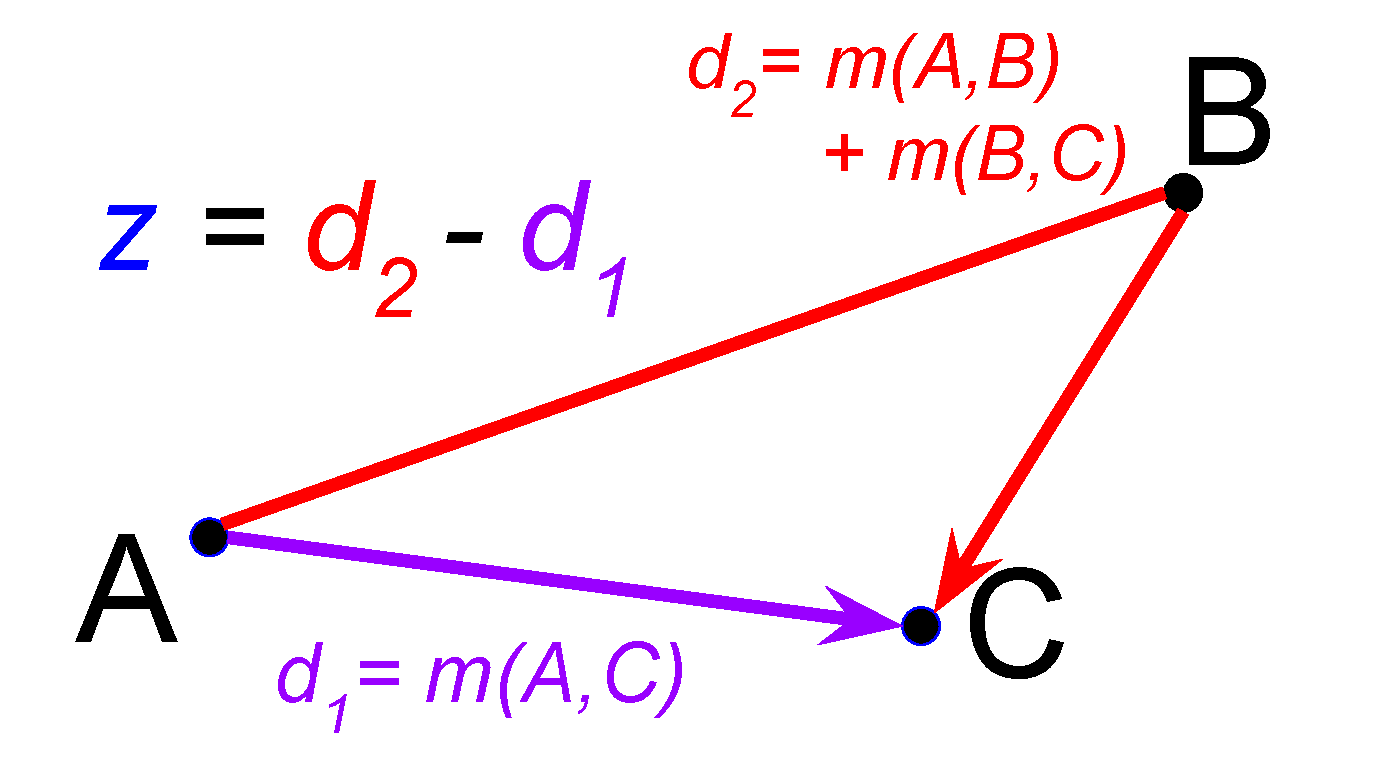
\includegraphics[width=\linewidth,trim=2cm 5cm 2cm 5cm, clip]{detour-difference}
\end{center}
\end{minipage}%
\begin{minipage}{0.5\textwidth}
\caption{
Sampling process used to evaluate detour difference, $z$.
} \label{fig:detour_difference_cartoon}
\end{minipage}
\end{subfigure}
\end{minipage}

\begin{minipage}{\linewidth}
\begin{subfigure}[b]{\linewidth}
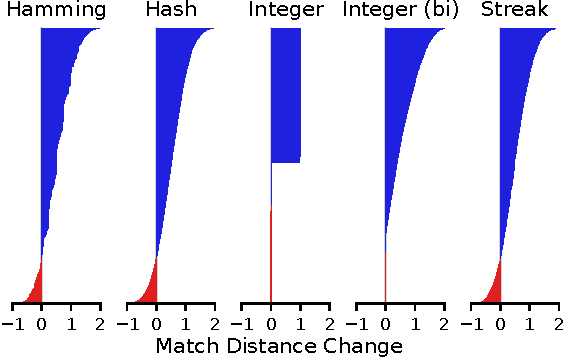
\includegraphics[width=\linewidth]{detour_difference/bitweight=0dot5+seed=1+title=low-triplet-analysis+_data_hathash_hash=6b0749ef97a58721+_script_fullcat_hash=297c4fe09078e17b+ext=}
\caption{
Distributions of detour distance difference for triplets of randomly sampled tags.
Each bar sliver represents an independently sampled observation.
A positive value (colored blue) indicates that total distance increased with the addition of an intermediate stop.
A value of exactly 0 indicates an intermediate stop had no effect on total distance.
A negative value (colored red) indicates violation of the triangle inequality: taking an intermediate stop reduced the total distance travelled.
} \label{fig:detour_difference_distribution}

\end{subfigure}
\end{minipage}

\caption{
Detour difference of tag-matching metrics.
}
\label{fig:detour_difference}

\end{center}
\end{figure}


To get a sense of the regularity, in a looses sense, of each space we uniformly sampled triplets of points $A$, $B$, and $C$.
Then, for each metric $m$ we calculated the statistic $m(A, B) + m(B, C) - m(A, C)$.
If the triangle inequality is respected this statistic should be greater than or equal to zero.
Figure \ref{fig:detour_difference} plots the distribution of this statistic for each metric.
The hamming, hash, and streak metrics show evidence of ``shortcuts'' that violate the triangle inequality.
It should be noted that the raw hamming metric does respect the triangle inequality.



